\section*{Author Information}

\noindent\begin{minipage}{0.22\linewidth}
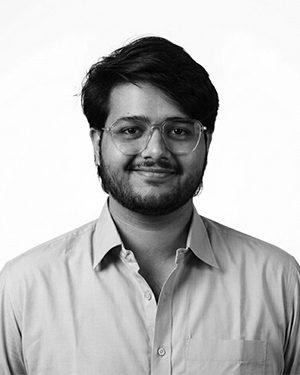
\includegraphics[width=\linewidth,clip,keepaspectratio]{a2.png}
\end{minipage}\hfill
\begin{minipage}{0.74\linewidth}
\textbf{Lakshya} is currently pursuing his M.Tech. in Artificial Intelligence and Machine Learning at Manipal University Jaipur, having completed his B.Tech. in Computer Science and Engineering from SRMIST, Chennai. His research interests include Multimodal Representation Learning, Computer Vision, Knowledge Distillation, and High-Performance AI Systems. He has authored research works currently in pipeline, including studies on modality dominance mitigation in unified multi modal learning and cost-efficient edge deployment of deep learning models through knowledge distillation and network pruning. As a systems engineer, he is the author of infergo (github.com/ailakshya/infergo), an open-source, production-grade AI inference runtime for Go, designed for framework-agnostic model serving across LLMs, computer vision, and general ML workloads. He is proficient in Python, Go, and C++, with practical expertise in CUDA optimization, MLOps, Explainable AI, and distributed inference systems. His work consistently bridges academic research and production engineering, with applications spanning healthcare, agriculture, and AI infrastructure.
\end{minipage}

\vspace{1em}

\noindent\begin{minipage}{0.22\linewidth}
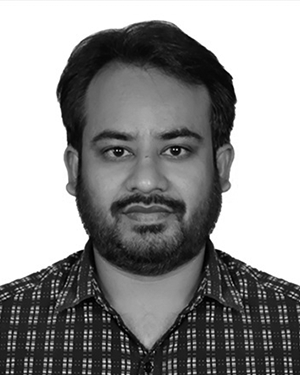
\includegraphics[width=\linewidth,clip,keepaspectratio]{a1.png}
\end{minipage}\hfill
\begin{minipage}{0.74\linewidth}
\textbf{Amit Kumar Bairwa} serves as a distinguished academician in the School of Computer Science and Engineering at Manipal University Jaipur. He holds an impressive academic background, boasting qualifications such as B.E., M.Tech., and Ph.D. in Computer Science and Engineering. His expertise lies in the fields of Optimization, MANET, Network Security, Machine Learning. As an accomplished author, Dr. Bairwa has published 4 books and is actively involved in research across various areas of his interest. He is a valued member of prestigious organizations including ISTE, ACM, and IEEE, which reflects his commitment to professional growth and networking. In addition to his academic pursuits, Dr. Amit is highly proficient in handling real-time challenges related to network and Linux-based systems. He has earned several international certifications, such as CCNA, RHCE, and CEH, demonstrating his dedication to staying current with the latest industry practices. Dr. Amit also designed 4 grants and 8 copyrights. Furthermore, Dr. Bairwa has made significant contributions to the academic ecosystem during his tenure. His approach involves a well-balanced combination of theoretical concepts and industry-oriented training modules. Collaborating with fellow academicians, Dr. Amit Kumar Bairwa has played an integral role in setting and maintaining high curriculum standards. He actively contributes to the development of mission statements and establishes performance goals and objectives, ensuring that the educational institution consistently excels in its academic pursuits.
\end{minipage}

\vspace{1em}

\noindent\begin{minipage}{0.22\linewidth}
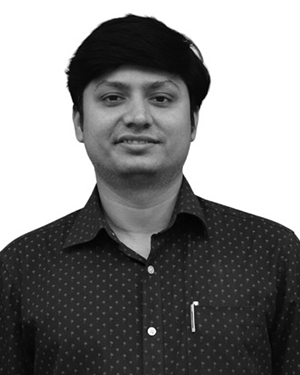
\includegraphics[width=\linewidth,clip,keepaspectratio]{a3.png}
\end{minipage}\hfill
\begin{minipage}{0.74\linewidth}
\textbf{Varun Tiwari} is a distinguished academician at the School of Computer Science and Engineering, Manipal University Jaipur. He holds a Ph.D. from Rajasthan Technical University Kota, and both a B.Tech. and M.Tech. in Computer Science and Engineering. His research expertise lies in Image Processing and Machine Learning, where he is known for his innovative solutions to complex problems. Dr. Tiwari has authored four books and published extensively in leading journals and conferences. He is a member of ACM and IEEE, reflecting his commitment to his field. Notable for his work in Image Processing, Machine Learning, and Computer Vision, Dr. Tiwari has made significant contributions to enhancing academic programs and aligning them with industry needs. He is also the organizer of the International Conference on Computation of Artificial Intelligence \& Machine Learning (ICCAIML) and actively participates in workshops and academic events.
\end{minipage}
